\documentclass[11pt]{article}
\usepackage[top=1cm, bottom=2cm, left=1cm, right=1cm]{geometry}
\usepackage{ctex}
\usepackage[linesnumbered,ruled]{algorithm2e}
\usepackage{amsthm,amsmath,amssymb}
\usepackage[colorlinks=true,linkcolor=blue]{hyperref}
\usepackage{listings}
\usepackage{xcolor,xparse}
\usepackage{realboxes}
\usepackage{mathrsfs}
\usepackage{wrapfig}
\usepackage{subfigure}
\usepackage{forest}
\usepackage{pifont}
\usepackage{tikz}
\usepackage{float}

\SetKw{Print}{print}
\SetKw{Read}{read}
\SetKw{Allocate}{allocate}
\SetKw{Deallocate}{deallocate}
\SetKw{Call}{call}
\SetKw{True}{true}
\SetKw{False}{false}
\SetKw{Continue}{continue}
\SetKw{Break}{break}
\SetKw{Write}{write}

\definecolor{cmdbg}{rgb}{0.9,0.9,0.9}
\lstset{%
	basicstyle=\ttfamily,
	breaklines = true,
	backgroundcolor=\color{cmdbg},
}
\DeclareDocumentCommand{\ccmd}{v}{% 参数 v 表示工作方法类似于 \verb
    \Colorbox{cmdbg}{\csname lstinline\endcsname!#1!}%
}


\author{杨远青 22300190015}
\title{计算物理作业2}

\begin{document}
\maketitle

\section{题目 1:三次方程根的求解与精确化}
\subsection{题目描述}
\noindent Write a code to numerically solves the motion of a simple pendulum using \textbf{Euler's method, midpoint method, RK4 method} and \textbf{Euler-trapezoidal method} (implement these methods by yourself). Plot the angle and total energy as a function of time. Explain the results.

\subsection{程序描述}
本程序内置了一个Pendulum类,具有绳长,质量(小球视作质点),初始角度,初始角速度,重力加速度等属性。通过调用Pendulum类的方法,可以使用Euler's method, midpoint method, RK4 method和Euler-trapezoidal method来求解简单摆的运动,会返回角度与角速度的numpy数组。类的方法还包括辅助的导数计算,即演化方程
\[
\begin{aligned}
\frac{d\theta}{dt} &= \omega, \\
\frac{d\omega}{dt} &= -\frac{g}{L} \sin(\theta),
\end{aligned}
\]
与总能量采集方法
\[
E = T + V = \frac{1}{2} m (\omega L)^2+ m g L (1 - \cos\theta)
\]
主程序还有内置的解析解、误差计算与用户输入采集函数,其中解析解借助了\texttt{scipy.special}的雅可比椭圆积分\texttt{sn,cn},模数$k = \sin(\theta_0/2)$,固有频率$\omega_0 = \sqrt{\frac{g}{L}}$,所以对大角度的摆动也是精确的。
\[
\theta(t) = 2 \arcsin\left(k \, \text{sn}(\omega_0 t + \frac{\pi}{2}, k^2)\right)
\]
\[
\omega(t) = \frac{2 k \omega_0 \, \text{cn}(\omega_0 t + \frac{\pi}{2}, k^2)}{\sqrt{1 - k^2 \, \text{sn}^2(\omega_0 t + \frac{\pi}{2}, k^2)}}
\]

\subsubsection{欧拉法 (Euler’s Method)}

\[
\begin{aligned}
\theta_{i+1} &= \theta_i + h \cdot \frac{d\theta}{dt} \bigg|_{t_i} \quad
\omega_{i+1} = \omega_i + h \cdot \frac{d\omega}{dt} \bigg|_{t_i}
\end{aligned}
\]

\subsubsection{中点法 (Midpoint Method)}

\[
\begin{aligned}
\text{计算中点值:} \quad
\theta_{\text{mid}} &= \theta_i + \frac{h}{2} \cdot \frac{d\theta}{dt} \bigg|_{t_i}, \quad
\omega_{\text{mid}} = \omega_i + \frac{h}{2} \cdot \frac{d\omega}{dt} \bigg|_{t_i} \\
\text{使用中点斜率更新:} \quad
\theta_{i+1} &= \theta_i + h \cdot \frac{d\theta}{dt} \bigg|_{\text{mid}}, \quad
\omega_{i+1} = \omega_i + h \cdot \frac{d\omega}{dt} \bigg|_{\text{mid}}
\end{aligned}
\]

\subsubsection{四阶龙格-库塔法 (RK4 Method)}

\[
\begin{aligned}
\text{第一步 (\(k_1\)):} \quad
k_1^\theta &= \frac{d\theta}{dt} \bigg|_{t_i, \theta_i, \omega_i}, \quad
k_1^\omega = \frac{d\omega}{dt} \bigg|_{t_i, \theta_i, \omega_i}; \\
\text{第二步 (\(k_2\)):} \quad
k_2^\theta &= \frac{d\theta}{dt} \bigg|_{t_i + \frac{h}{2}, \theta_i + \frac{h}{2} k_1^\theta, \omega_i + \frac{h}{2} k_1^\omega}, \quad 
k_2^\omega = \frac{d\omega}{dt} \bigg|_{t_i + \frac{h}{2}, \theta_i + \frac{h}{2} k_1^\theta, \omega_i + \frac{h}{2} k_1^\omega}; \\
\text{第三步 (\(k_3\)):} \quad
k_3^\theta &= \frac{d\theta}{dt} \bigg|_{t_i + \frac{h}{2}, \theta_i + \frac{h}{2} k_2^\theta, \omega_i + \frac{h}{2} k_2^\omega}, \quad
k_3^\omega = \frac{d\omega}{dt} \bigg|_{t_i + \frac{h}{2}, \theta_i + \frac{h}{2} k_2^\theta, \omega_i + \frac{h}{2} k_2^\omega}; \\
\text{第四步 (\(k_4\)):} \quad
k_4^\theta &= \frac{d\theta}{dt} \bigg|_{t_i + h, \theta_i + h k_3^\theta, \omega_i + h k_3^\omega}, \quad
k_4^\omega = \frac{d\omega}{dt} \bigg|_{t_i + h, \theta_i + h k_3^\theta, \omega_i + h k_3^\omega},;\\
\text{更新公式:} \quad
\theta_{i+1} &= \theta_i + \frac{h}{6} \left(k_1^\theta + 2k_2^\theta + 2k_3^\theta + k_4^\theta \right), \quad
\omega_{i+1} = \omega_i + \frac{h}{6} \left(k_1^\omega + 2k_2^\omega + 2k_3^\omega + k_4^\omega \right).
\end{aligned}
\]

\subsubsection{欧拉-梯形法 (Euler-Trapezoidal Method)}

\[
\begin{aligned}
\text{预测:} \quad
\theta_{\text{pred}} &= \theta_i + h \cdot \frac{d\theta}{dt} \bigg|_{t_i}, \quad
\omega_{\text{pred}} = \omega_i + h \cdot \frac{d\omega}{dt} \bigg|_{t_i} \\
\text{校正:} \quad
\theta_{i+1} &= \theta_i + \frac{h}{2} \left( \frac{d\theta}{dt} \bigg|_{t_i} + \frac{d\theta}{dt} \bigg|_{\text{pred}} \right) \quad
\omega_{i+1} = \omega_i + \frac{h}{2} \left( \frac{d\omega}{dt} \bigg|_{t_i} + \frac{d\omega}{dt} \bigg|_{\text{pred}} \right)
\end{aligned}
\]
\subsection{伪代码}
Powered by \href{https://chatgpt.com/g/g-xJJAA2awf-latex-pseudocode-generator}{\LaTeX \ pseudocode generator}

\begin{algorithm}[H]
    \SetAlgoLined
    \SetKwFunction{Derivatives}{Derivatives}
    \KwIn{$h$: Time step size (float), $N$: Total number of steps (int)}
    \KwOut{$\theta$: Angle array (rad), $\omega$: Angular velocity array (rad/s)}
    
    Initialize $\theta[0] \gets \theta_0$, $\omega[0] \gets \omega_0$ \tcp*[r]{Set initial conditions}
    
    \For{$i \gets 0$ \KwTo $N-1$}{
        Compute $(\dot{\theta}, \dot{\omega}) \gets$ \Derivatives{$\theta[i], \omega[i]$}\;
        Update $\theta[i+1] \gets \theta[i] + h \cdot \dot{\theta}$, $\omega[i+1] \gets \omega[i] + h \cdot \dot{\omega}$ \tcp*[r]{Update values}
    }
    
    \KwRet{$\theta, \omega$} \tcp*[r]{Return results as arrays}
    \caption{Euler Method for Simple Harmonic Oscillator}
\end{algorithm}
\begin{algorithm}[H]
        \SetAlgoLined
        \SetKwFunction{Derivatives}{Derivatives}
        \KwIn{$h$: Time step size (float), $N$: Total number of steps (int)}
        \KwOut{$\theta$: Angle array (rad), $\omega$: Angular velocity array (rad/s)}
        
        Initialize $\theta[0] \gets \theta_0$, $\omega[0] \gets \omega_0$ \tcp*[r]{Set initial conditions}
        
        \For{$i \gets 0$ \KwTo $N-1$}{
            Compute $(\dot{\theta}, \dot{\omega}) \gets$ \Derivatives{$\theta[i], \omega[i]$} \tcp*[r]{Slope at initial point}
            Compute $\theta_{\text{mid}} \gets \theta[i] + 0.5 \cdot h \cdot \dot{\theta}$, $\omega_{\text{mid}} \gets \omega[i] + 0.5 \cdot h \cdot \dot{\omega}$ \tcp*[r]{Midpoint values}
        
            Compute $(\dot{\theta}_{\text{mid}}, \dot{\omega}_{\text{mid}}) \gets$ \Derivatives{$\theta_{\text{mid}}, \omega_{\text{mid}}$} \tcp*[r]{Slope at midpoint}
            Update $\theta[i+1] \gets \theta[i] + h \cdot \dot{\theta}_{\text{mid}}$, $\omega[i+1] \gets \omega[i] + h \cdot \dot{\omega}_{\text{mid}}$ \tcp*[r]{Update values}
        }
        
        \KwRet{$\theta, \omega$} \tcp*[r]{Return results as arrays}
        \caption{Midpoint Method for Simple Harmonic Oscillator}
\end{algorithm}
\begin{algorithm}[H]
    \SetAlgoLined
    \SetKwFunction{Derivatives}{Derivatives}
    \KwIn{$h$: Time step size (float), $N$: Total number of steps (int)}
    \KwOut{$\theta$: Angle array (rad), $\omega$: Angular velocity array (rad/s)}
    
    Initialize $\theta[0] \gets \theta_0$, $\omega[0] \gets \omega_0$ \tcp*[r]{Set initial conditions}
    
    \For{$i \gets 0$ \KwTo $N-1$}{
        Compute $(k_1^\theta, k_1^\omega) \gets$ \Derivatives{$\theta[i], \omega[i]$} \tcp*[r]{Stage 1}
        Compute $(k_2^\theta, k_2^\omega) \gets$ \Derivatives{$\theta[i] + 0.5 \cdot h \cdot k_1^\theta, \omega[i] + 0.5 \cdot h \cdot k_1^\omega$} \tcp*[r]{Stage 2}
        Compute $(k_3^\theta, k_3^\omega) \gets$ \Derivatives{$\theta[i] + 0.5 \cdot h \cdot k_2^\theta, \omega[i] + 0.5 \cdot h \cdot k_2^\omega$} \tcp*[r]{Stage 3}
        Compute $(k_4^\theta, k_4^\omega) \gets$ \Derivatives{$\theta[i] + h \cdot k_3^\theta, \omega[i] + h \cdot k_3^\omega$} \tcp*[r]{Stage 4}
    
        Update $\theta[i+1] \gets \theta[i] + \frac{h}{6} \cdot (k_1^\theta + 2 \cdot k_2^\theta + 2 \cdot k_3^\theta + k_4^\theta)$\;
        Update $\omega[i+1] \gets \omega[i] + \frac{h}{6} \cdot (k_1^\omega + 2 \cdot k_2^\omega + 2 \cdot k_3^\omega + k_4^\omega)$\;
    }
    
    \KwRet{$\theta, \omega$} \tcp*[r]{Return results as arrays}
    \caption{RK4 Method for Simple Harmonic Oscillator}
\end{algorithm}
\begin{algorithm}[H]
            \SetAlgoLined
            \SetKwFunction{Derivatives}{Derivatives}
            \KwIn{$h$: Time step size (float), $N$: Total number of steps (int)}
            \KwOut{$\theta$: Angle array (rad), $\omega$: Angular velocity array (rad/s)}
            
            Initialize $\theta[0] \gets \theta_0$, $\omega[0] \gets \omega_0$ \tcp*[r]{Set initial conditions}
            
            \For{$i \gets 0$ \KwTo $N-1$}{
                Compute $(\dot{\theta}, \dot{\omega}) \gets$ \Derivatives{$\theta[i], \omega[i]$} \tcp*[r]{Predictor step slopes}
                Compute $\theta_{\text{pred}} \gets \theta[i] + h \cdot \dot{\theta}$, $\omega_{\text{pred}} \gets \omega[i] + h \cdot \dot{\omega}$ \tcp*[r]{Euler predictor values}
            
                Compute $(\dot{\theta}_{\text{pred}}, \dot{\omega}_{\text{pred}}) \gets$ \Derivatives{$\theta_{\text{pred}}, \omega_{\text{pred}}$} \tcp*[r]{Corrector step slopes}
                Update $\theta[i+1] \gets \theta[i] + \frac{h}{2} \cdot (\dot{\theta} + \dot{\theta}_{\text{pred}})$, $\omega[i+1] \gets \omega[i] + \frac{h}{2} \cdot (\dot{\omega} + \dot{\omega}_{\text{pred}})$ \tcp*[r]{Trapezoidal corrector}
            }
            
            \KwRet{$\theta, \omega$} \tcp*[r]{Return results as arrays}
            \caption{Euler-Trapezoidal Method for Simple Harmonic Oscillator}
\end{algorithm}
\subsection{结果示例}
\begin{figure}[H]
    \centering
    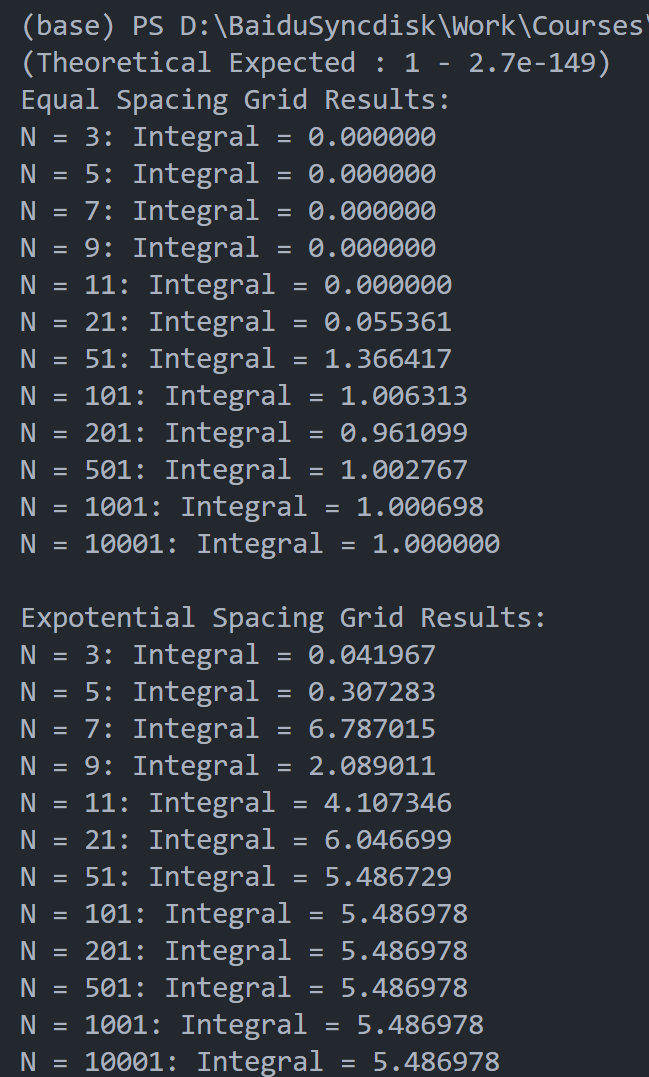
\includegraphics[width=1.0\textwidth]{Problem_1/figs/terminal.png}
    \caption{终端处理用户输入,此处均采用默认值}
\end{figure}
\begin{figure}[H]
    \centering
    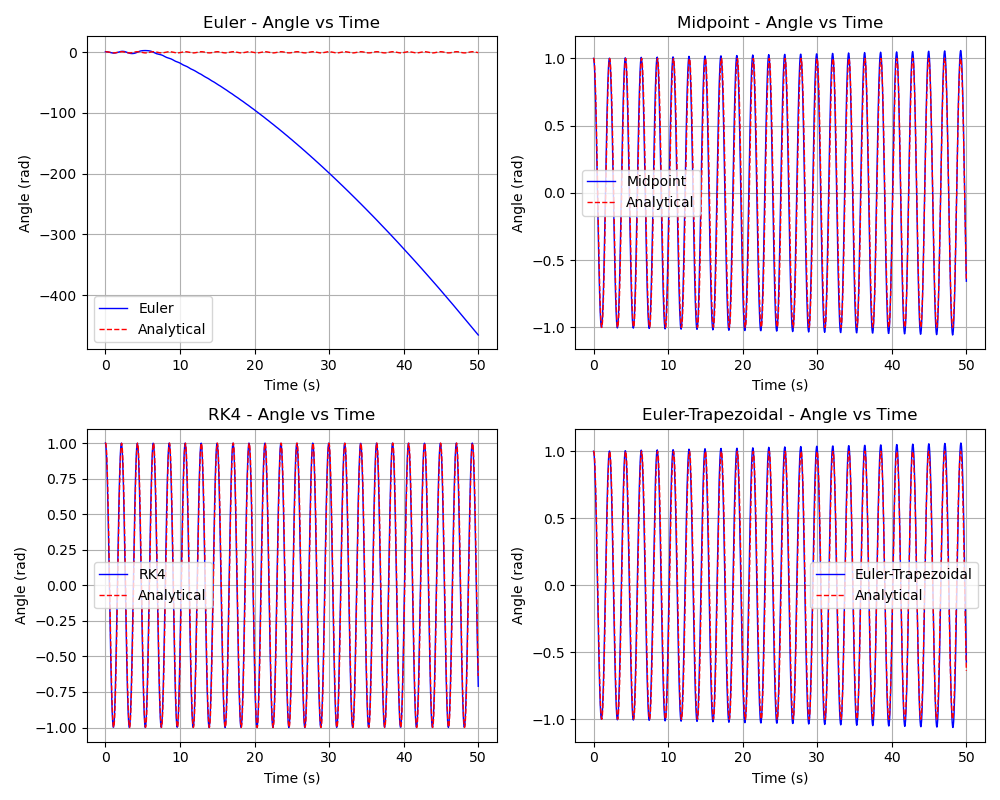
\includegraphics[width=1.0\textwidth]{Problem_1/figs/angle_time.png}
    \caption{角度随时间变化}
\end{figure}
\begin{figure}[H]
    \centering
    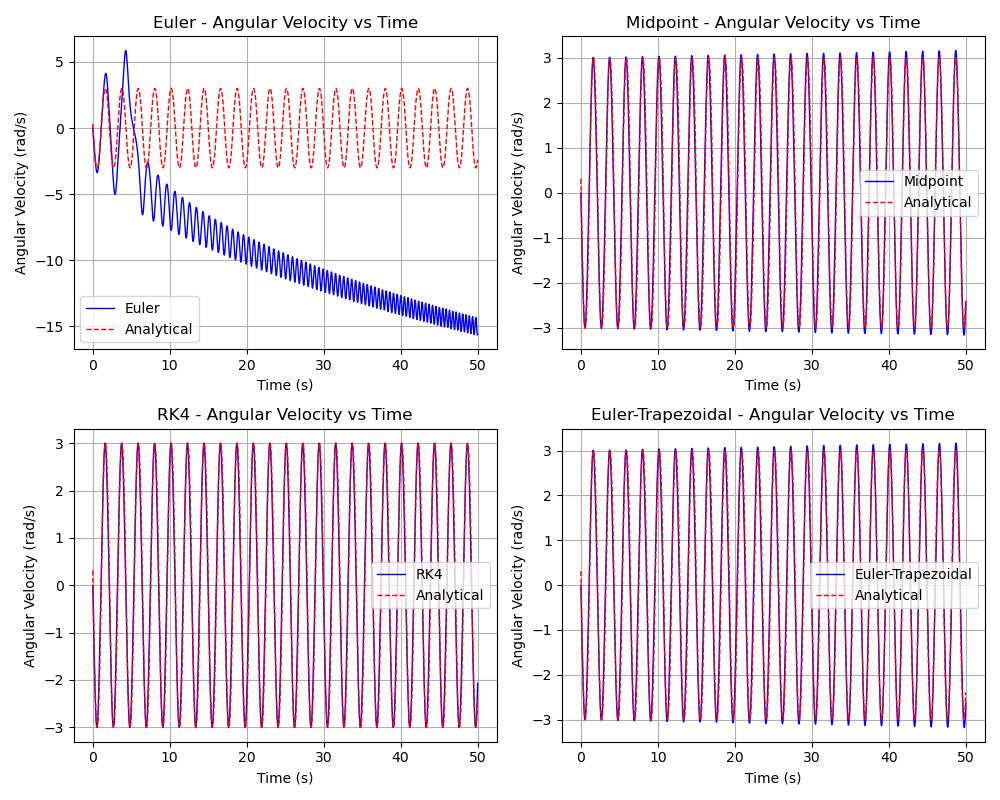
\includegraphics[width=1.0\textwidth]{Problem_1/figs/angle_velocity_time.png}
    \caption{角速度随时间变化}
\end{figure}
\begin{figure}[H]
    \centering
    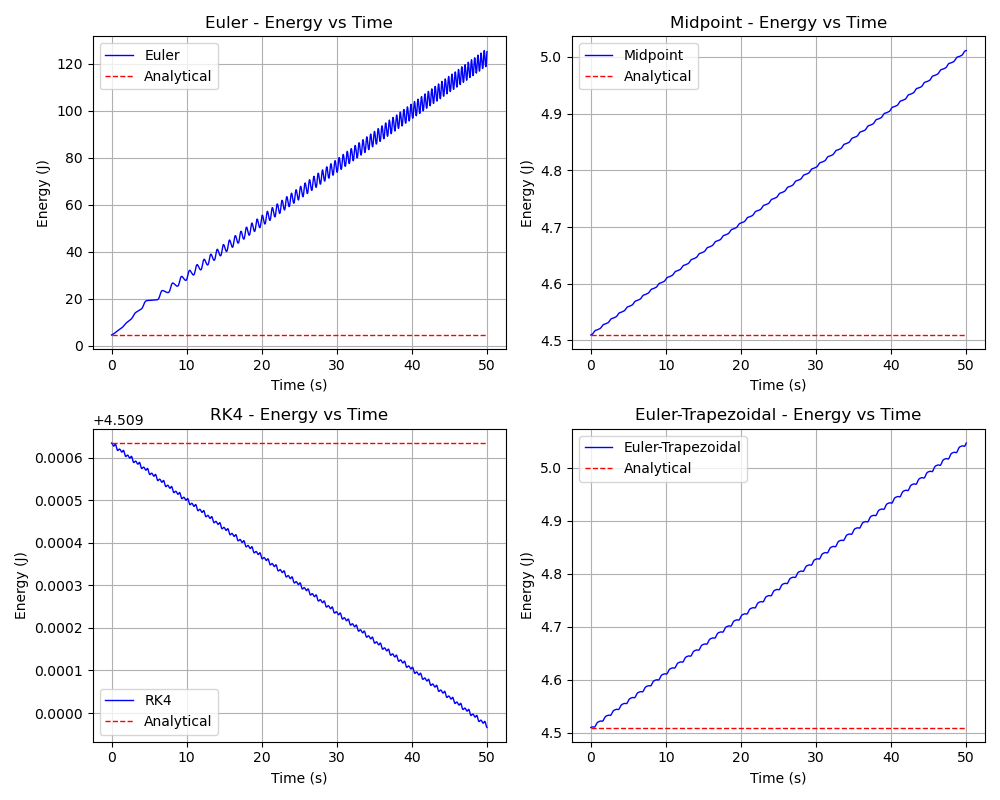
\includegraphics[width=1.0\textwidth]{Problem_1/figs/energy_time.png}
    \caption{能量随时间漂移}
\end{figure}
\begin{figure}[H]
    \centering
    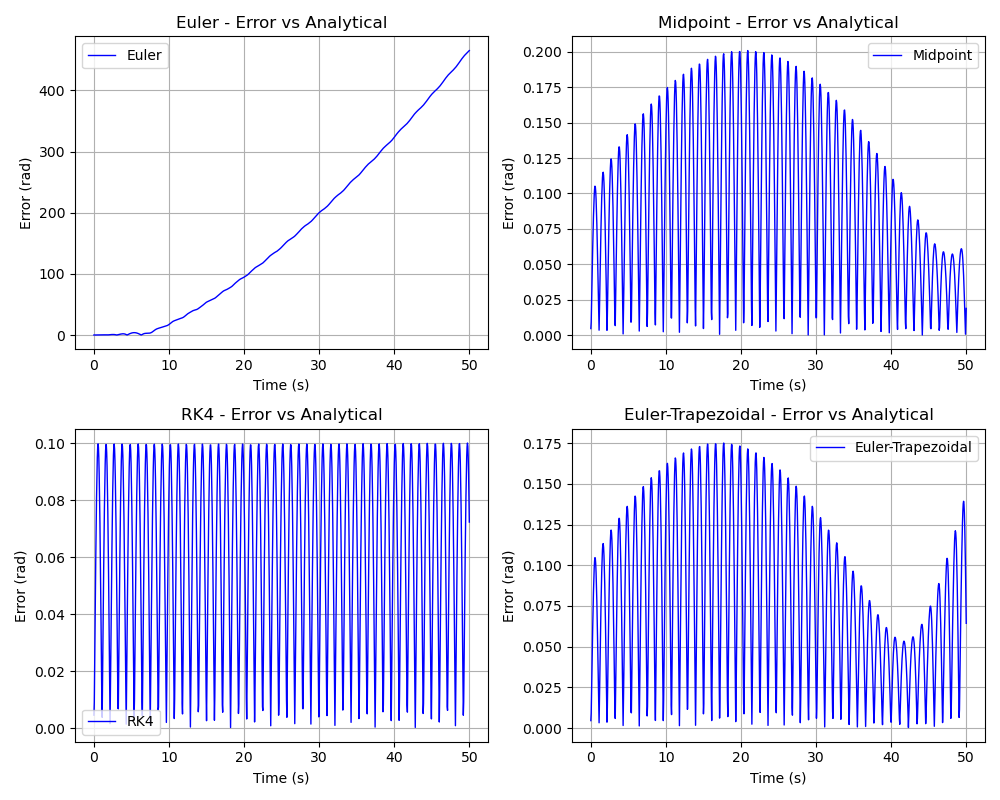
\includegraphics[width=1.0\textwidth]{Problem_1/figs/angle_error_time.png}
    \caption{角度与解析解误差随时间变化}
\end{figure}
可以看出,四种方法对比中,RK4方法的能量漂移最小,角度与角速度误差也最小。中点法与欧拉-梯形法次之,虽然角度、角速度误差在长时间后才逐渐显现,但能量漂移较大。欧拉法误差最大,一段时间后就崩溃。综上,RK4方法最为精确且稳定。

\section{题目 2:二维函数的极小值搜索}
\subsection{题目描述}
\noindent Write a code to numerically solve the radial Schrödinger equation for
\[
\left[-\frac{1}{2}\nabla^2+V(\mathbf{r})\right]\psi(\mathbf{r})=E\psi(\mathbf{r}), \quad V(\mathbf{r})=V(r)
\]
\begin{enumerate}
    \item \( V(r) = \frac{1}{r} \) (hydrogen atom)
    \item Considering the following potential:
    \[
    V(r) = -\frac{Z_{\text{ion}}}{r}\text{erf}\left(\frac{r}{\sqrt{2} r_{\text{loc}}}\right) 
    + \exp \left[ -\frac{1}{2} \left(\frac{r}{r_{\text{loc}}}\right)^{\frac{1}{2}}\right]
    \times \left[C_1 + C_2\left(\frac{r}{r_{\text{loc}}}\right)^2+C_3\left(\frac{r}{r_{\text{loc}}}\right)^4+C_4\left(\frac{r}{r_{\text{loc}}}\right)^6\right]
    \]
\end{enumerate}
where \(\text{erf}\) is the error function. And for Li, you could set:
\begin{itemize}
    \item \( Z_{\text{ion}}=3 \)
    \item \( r_{\text{loc}}=0.4 \)
    \item \( C_1=-14.0093922 \)
    \item \( C_2=9.5099073 \)
    \item \( C_3=-1.7532723 \)
    \item \( C_4=0.0834586 \)
\end{itemize}
\noindent Compute and plot the first three eigenstates. You could find more information about 'how to solve radial Schrödinger equation' and 'use of non-uniform grid (optional)' in the PPT.

\textbf{Special Note:} You may call any library functions for diagonalization.


\subsection{程序描述}

\subsection{伪代码}
Powered by \href{https://chatgpt.com/g/g-xJJAA2awf-latex-pseudocode-generator}{\LaTeX \ pseudocode generator}

\subsection{结果示例}



\section{题目 3:有限深方势阱中的电子能级与波函数}
\subsection{题目描述}
\noindent Given \( n+1 \) points \((x_0, y_0), (x_1, y_1), \dots, (x_n, y_n)\), the \( n \)-th order interpolation polynomial using Newton's method is:
\[
P_n(x) = f[x_0] + f[x_1, x_0](x - x_0) + f[x_2, x_1, x_0](x - x_0)(x - x_1) + \cdots + f[x_n, x_{n-1}, \dots, x_0](x - x_0)(x - x_1) \dots (x - x_{n-1})
\]
where \( f[x_i, x_{i-1}, \dots, x_0] \) represents the divided differences. Taking the coefficients from the lower edge of the difference table (i.e., \( f[x_n], f[x_n, x_{n-1}], \dots, f[x_n, \dots, x_0] \)), will this provide higher accuracy for values of \( x \) near \( x_n \)?

\begin{center}
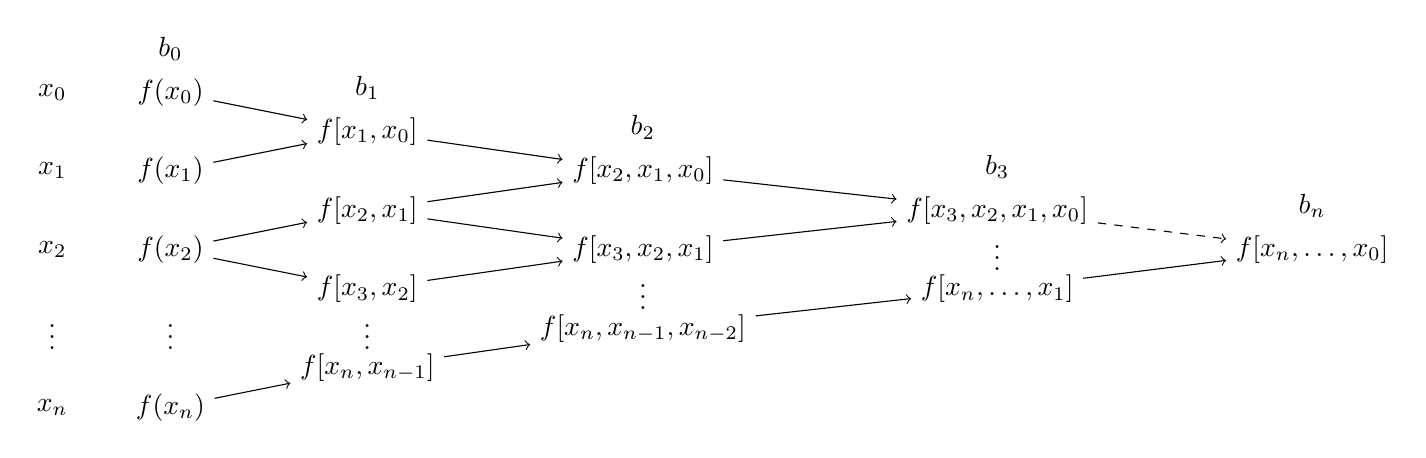
\begin{tikzpicture}
    % Column 1 (x values)
    \node (x0) at (-4, 0) {$x_0$};
    \node (x1) at (-4, -1) {$x_1$};
    \node (x2) at (-4, -2) {$x_2$};
    \node (dots) at (-4, -3) {$\vdots$};
    \node (xn) at (-4, -4) {$x_n$};

    % Column 2 (f(x) values)
    \node (f0) at (-2.5, 0) {$f(x_0)$};
    \node (f1) at (-2.5, -1) {$f(x_1)$};
    \node (f2) at (-2.5, -2) {$f(x_2)$};
    \node (fdots) at (-2.5, -3) {$\vdots$};
    \node (fn) at (-2.5, -4) {$f(x_n)$};

    % Column 3 (f[x1, x0], etc.)
    \node (f10) at (0, -0.5) {$f[x_1, x_0]$};
    \node (f21) at (0, -1.5) {$f[x_2, x_1]$};
    \node (f32) at (0, -2.5) {$f[x_3, x_2]$};
    \node (fdots2) at (0, -3) {$\vdots$};
    \node (fnn1) at (0, -3.5) {$f[x_n, x_{n-1}]$};

    % Column 4 (f[x2, x1, x0], etc.)
    \node (f210) at (3.5, -1) {$f[x_2, x_1, x_0]$};
    \node (f321) at (3.5, -2) {$f[x_3, x_2, x_1]$};
    \node (fdots3) at (3.5, -2.5) {$\vdots$};
    \node (fnnn2) at (3.5, -3) {$f[x_n, x_{n-1}, x_{n-2}]$};

    % Column 5 (f[x3, x2, x1, x0], etc.)
    \node (f3210) at (8, -1.5) {$f[x_3, x_2, x_1, x_0]$};
    \node (fdots4) at (8, -2) {$\vdots$};
    \node (fnnnn3) at (8, -2.5) {$f[x_n, \dots, x_1]$};

    % Column 6 (final term)
    \node (final) at (12, -2) {$f[x_n, \dots, x_0]$};

    % Labels for coefficients
    \node[above=8pt] at (f0) {$b_0$}; % 向上偏移8pt
    \node[above=8pt] at (f10) {$b_1$};
    \node[above=8pt] at (f210) {$b_2$};
    \node[above=8pt] at (f3210) {$b_3$};
    \node[above=8pt] at (final) {$b_n$};

    % Drawing connections with (dashed) lines
    \draw[->] (f0) -- (f10);
    \draw[->] (f10) -- (f210);
    \draw[->] (f210) -- (f3210);
    \draw[dashed, ->] (f3210) -- (final);

    % Drawing vertical solid lines within each column
    \draw[->] (f1) -- (f10);
    \draw[->] (f2) -- (f21);
    \draw[->] (f2) -- (f32);
    \draw[->] (f21) -- (f210);
    \draw[->] (f21) -- (f321);
    \draw[->] (f32) -- (f321);
    \draw[->] (f321) -- (f3210);
    \draw[->] (fn) -- (fnn1);
    \draw[->] (fnn1) -- (fnnn2);
    \draw[->] (fnnn2) -- (fnnnn3);
    \draw[->] (fnnnn3) -- (final);

\end{tikzpicture}
\end{center}

\subsection{程序描述}
原本对于不考虑舍入误差的理想形式,Newton插值与Lagrange插值的结果必定是唯一且等价的,也即通过给定$(n+1)$个节点的$n$阶多项式唯一,这一点可以从Vandermonde行列式
\[
\det \begin{pmatrix}
1 & x_0 & x_0^2 & \cdots & x_0^n \\
1 & x_1 & x_1^2 & \cdots & x_1^n \\
\vdots & \vdots & \vdots & & \vdots \\
1 & x_n & x_n^2 & \cdots & x_n^n
\end{pmatrix} = \prod_{0 \leq i < j \leq n} (x_j - x_i)
\]
非奇异中看出。但实际结果中,我们必须考虑舍入误差,这使得Newton插值的结果可能会依赖于节点的顺序。尤其是在我们使用Horner's Rule(\ref{eq:horner})的时候,显然在节点附近的插值数值稳定性依赖于节点的顺序。本程序使用\ref{sec:problem_1}节中的牛顿插值代码,对两个病态函数\(\mathrm{e}^x\)与\(\sin(100x)\)展开了数值实验。

实验中,我们分别在区间\([-10, 10]\)和\([-0.8, 0.5]\)上等距取25个节点,对两个函数进行顺序与逆序的牛顿插值,并在子图1中展示插值效果,在子图2中对比两者相较于真实函数的相对误差,在子图3中展示逆序插值与顺序插值相对误差的差值。在\(\mathrm{e}^x\)结果中使用了对数坐标轴以更好展示插值效果。
\subsection{实验结果}
\begin{figure}[H]
    \centering
    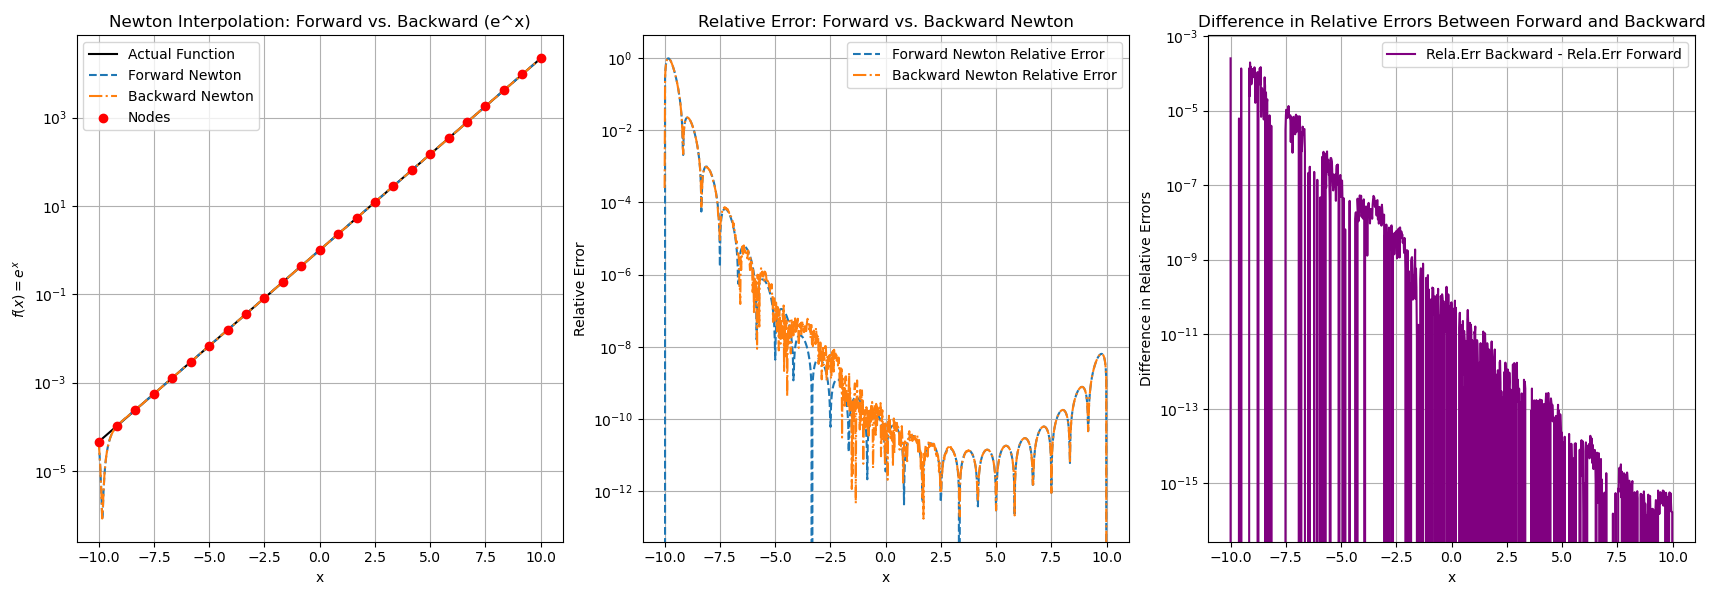
\includegraphics[width=1.0\textwidth]{Problem_3/figs/exp.png}
    \caption{\(\mathrm{e}^x\)实验结果}
\end{figure}
令人惊奇的是,对于病态函数\(\mathrm{e}^x\),顺序插值的效果始终优于逆序插值(表现为子图2中蓝色虚线始终位于橙色虚线下方,子图3中紫色曲线值始终非负)猜测可能是由于逆序差值的系数在计算初期便受到了较大的舍入误差的影响,而这种影响在Horner's Rule中被逐级放大,最终在传播后半段(子图左侧)逐渐显现。

\begin{figure}[H]
    \centering
    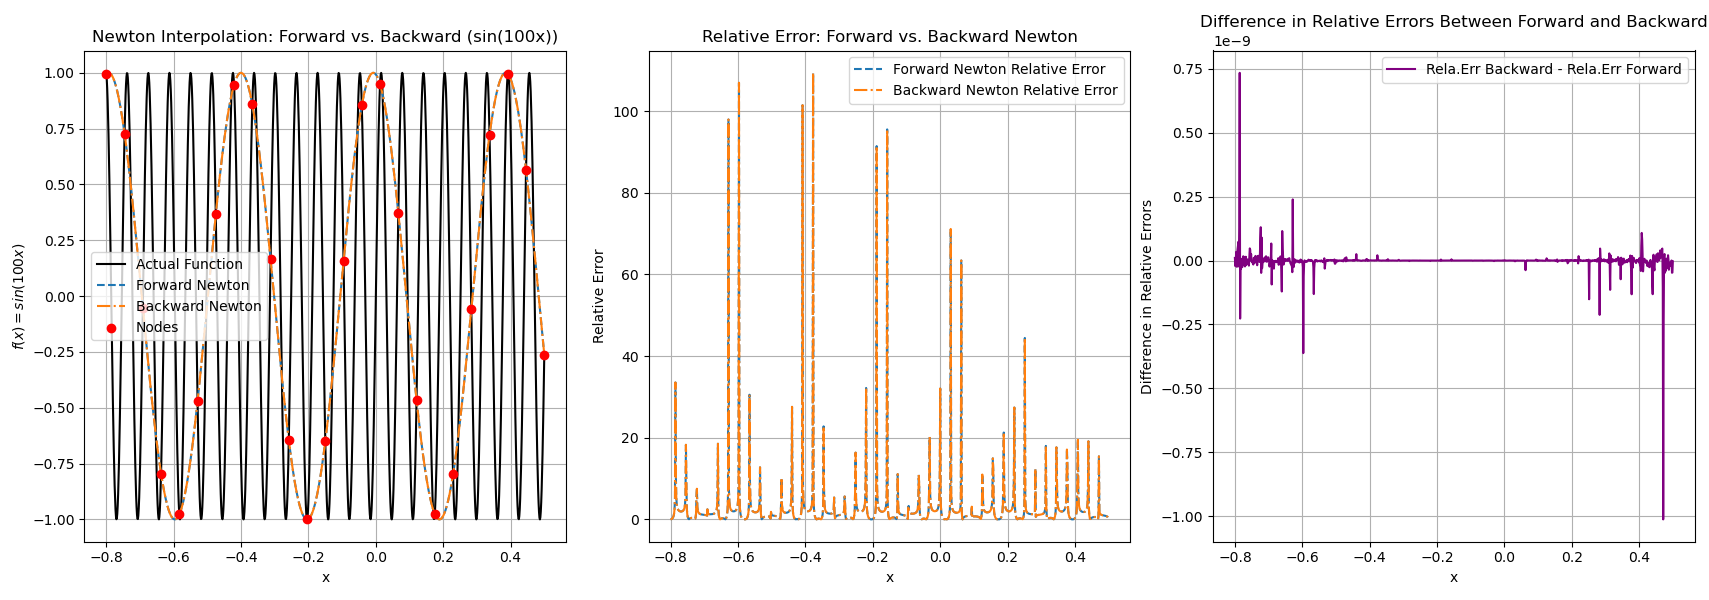
\includegraphics[width=1.0\textwidth]{Problem_3/figs/sin.png}
    \caption{\(\sin(100x)\)实验结果}
\end{figure}

对于高频震荡的病态函数\(\sin(100x)\),逆序差值与顺序差值这对卧龙凤雏,均展现了高达一倍以上的相对误差,相较于\(\mathrm{e}^x\)的结果,更为病态,也符合预期。令人惊喜的是,由于\(\sin(100x)\)本身的对称性与导数有界性,两种差值顺序的优劣对比在区间两端出现了符合预期的差别:在正向传播的末端(子图3右侧),顺序插值的相对误差超过了逆序差值,反之在另一侧,顺序差值结果更优,这符合我们最开始的朴素想法:随着节点的进行,舍入误差的影响逐渐增大,致使区间两侧效果不一,这也提示我们在边界附近应当采集更密的节点,如\ref{sec:problem_1}节中的Chebyshev与Leja节点。

\vspace{5pt}
\textit{今天原本应该是鏖战Griffths的猫与蔡先生的日子,可惜平板没电。}
\end{document}